%------------------------------------------------------------------------------%
% Luis A. D'Afonseca
%
% T1 - 28 alunos - 24T56
%------------------------------------------------------------------------------%
\documentclass[a4paper,12pt,fleqn]{article}

\usepackage{style_avaliacao}
\usepackage{graphicx}

\makeatletter
\graphicspath  {{./figs/}}
\def\input@path{{./figs/}}
\makeatother

\newcommand*{\prova}{Prova 1 -- Turma 4}
\newcommand*{\data}{31/08/2023}

%\usepackage{comment}
%\excludecomment{resposta}
\newenvironment{resposta}%
  {\begingroup\color{blue}\small\begin{spacing}{0.9}}%
  {\end{spacing}\endgroup}

%------------------------------------------------------------------------------%
\begin{document}

\makeHeader{Integrais e Séries}{\prova}{\data}

% 01
%------------------------------------------------------------------------------%
\exercise{25}
Dada a função
\(
  f(x) = \begin{cases}
    1-x^2,   & x < 0  \\
    \cos(x), & x \geq 0
  \end{cases}
\)
\begin{enumerate}[label=\alph*)]
  \item Esboce o gráfico de $f$
  \item Calcule \( \int f(x)\,dx \)
  \item Calcule \( \int_{-\pi}^\pi f(x)\,dx \)
\end{enumerate}

\begin{resposta}
\begin{enumerate}[label=\alph*)]
  \item (5 pontos)\\ 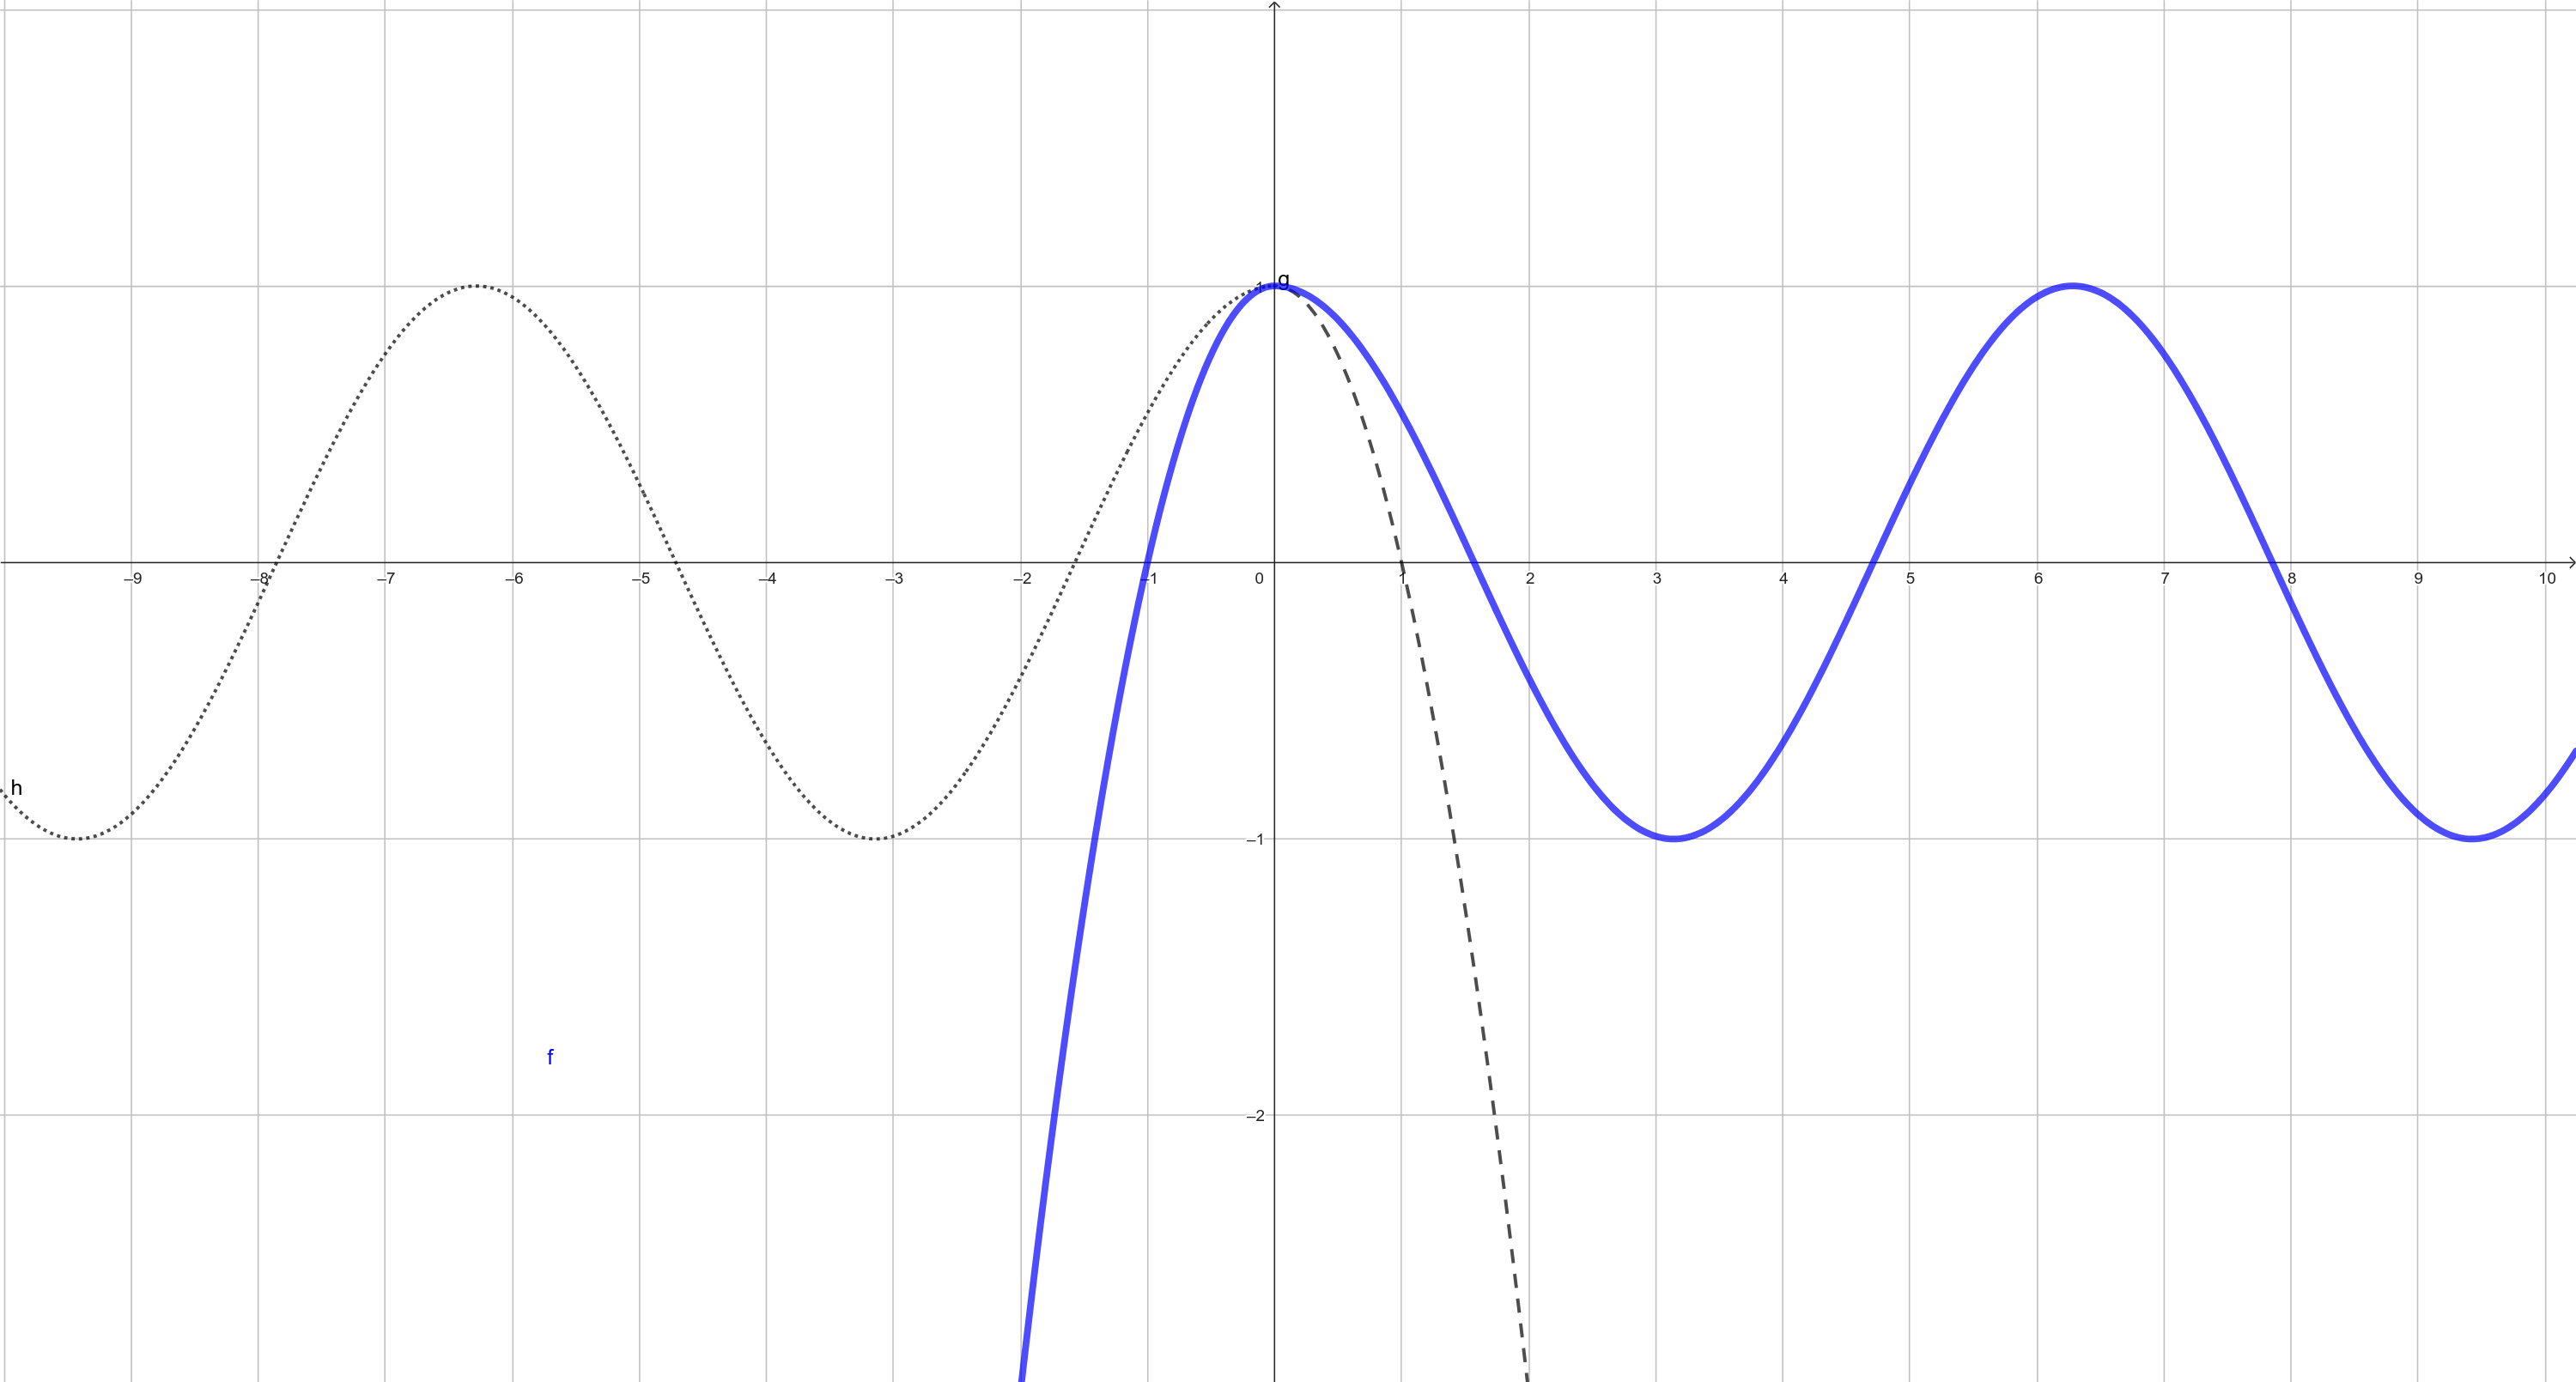
\includegraphics[height=6cm,width=\linewidth]{1_x2_cos}
  \item (10 pontos) \\
  Considerando o intervalo $(-\infty, 0)$, temos
  \[
    \int f(x)\, dx
    = \int 1-x^2\, dx
    = x - \frac{x^3}{3} + C
  \]
  No intervalo $[0, \infty)$, temos
  \[
  \int f(x)\, dx
  = \int \cos(x)\, dx
  = \sin(x) + C
  \]
  Portanto a primitiva de $f$ é
  \[
    F(x) = \begin{cases}
      x - \dfrac{x^3}{3} + C, & x < 0    \\[3mm]
      \sin(x) + C,            & x \geq 0
    \end{cases}
  \]

  \item (10 pontos) \\
  Para calcular a integral definida precisamos dividir o intervalo em duas partes
  \begin{align*}
    I
    & = \int_{-\pi}^\pi f(x)\,dx                         \\
    & = \int_{-\pi}^0 f(x)\,dx + \int_0^\pi f(x)\,dx     \\
    & = \int_{-\pi}^0 1-x^2\,dx + \int_0^\pi \cos(x)\,dx \\
    & = \left(x - \dfrac{x^3}{3}\right) \evalat{-\pi}{0}
      + \sin(x) \evalat{0}{\pi}                          \\
    & = 0 -\left((-\pi) - \frac{(-\pi)^3}{3}\right) + \sin(\pi) - \sin(0)     \\
    & = \pi - \frac{\pi^3}{3}
  \end{align*}
\end{enumerate}
\end{resposta}

% 02
%------------------------------------------------------------------------------%
\exercise{25}
Data a função \(f(x)=\frac{1}{\sqrt{x\,}}\)
\begin{enumerate}[label=\alph*)]
  \item Esboce o gráfico de $f$
  \item Calcule sua primitiva
  \item Calcule \( \int_0^4 f(x)\,dx \)
\end{enumerate}

\begin{resposta}
  \begin{enumerate}[label=\alph*)]
    \item(5 pontos) \\
    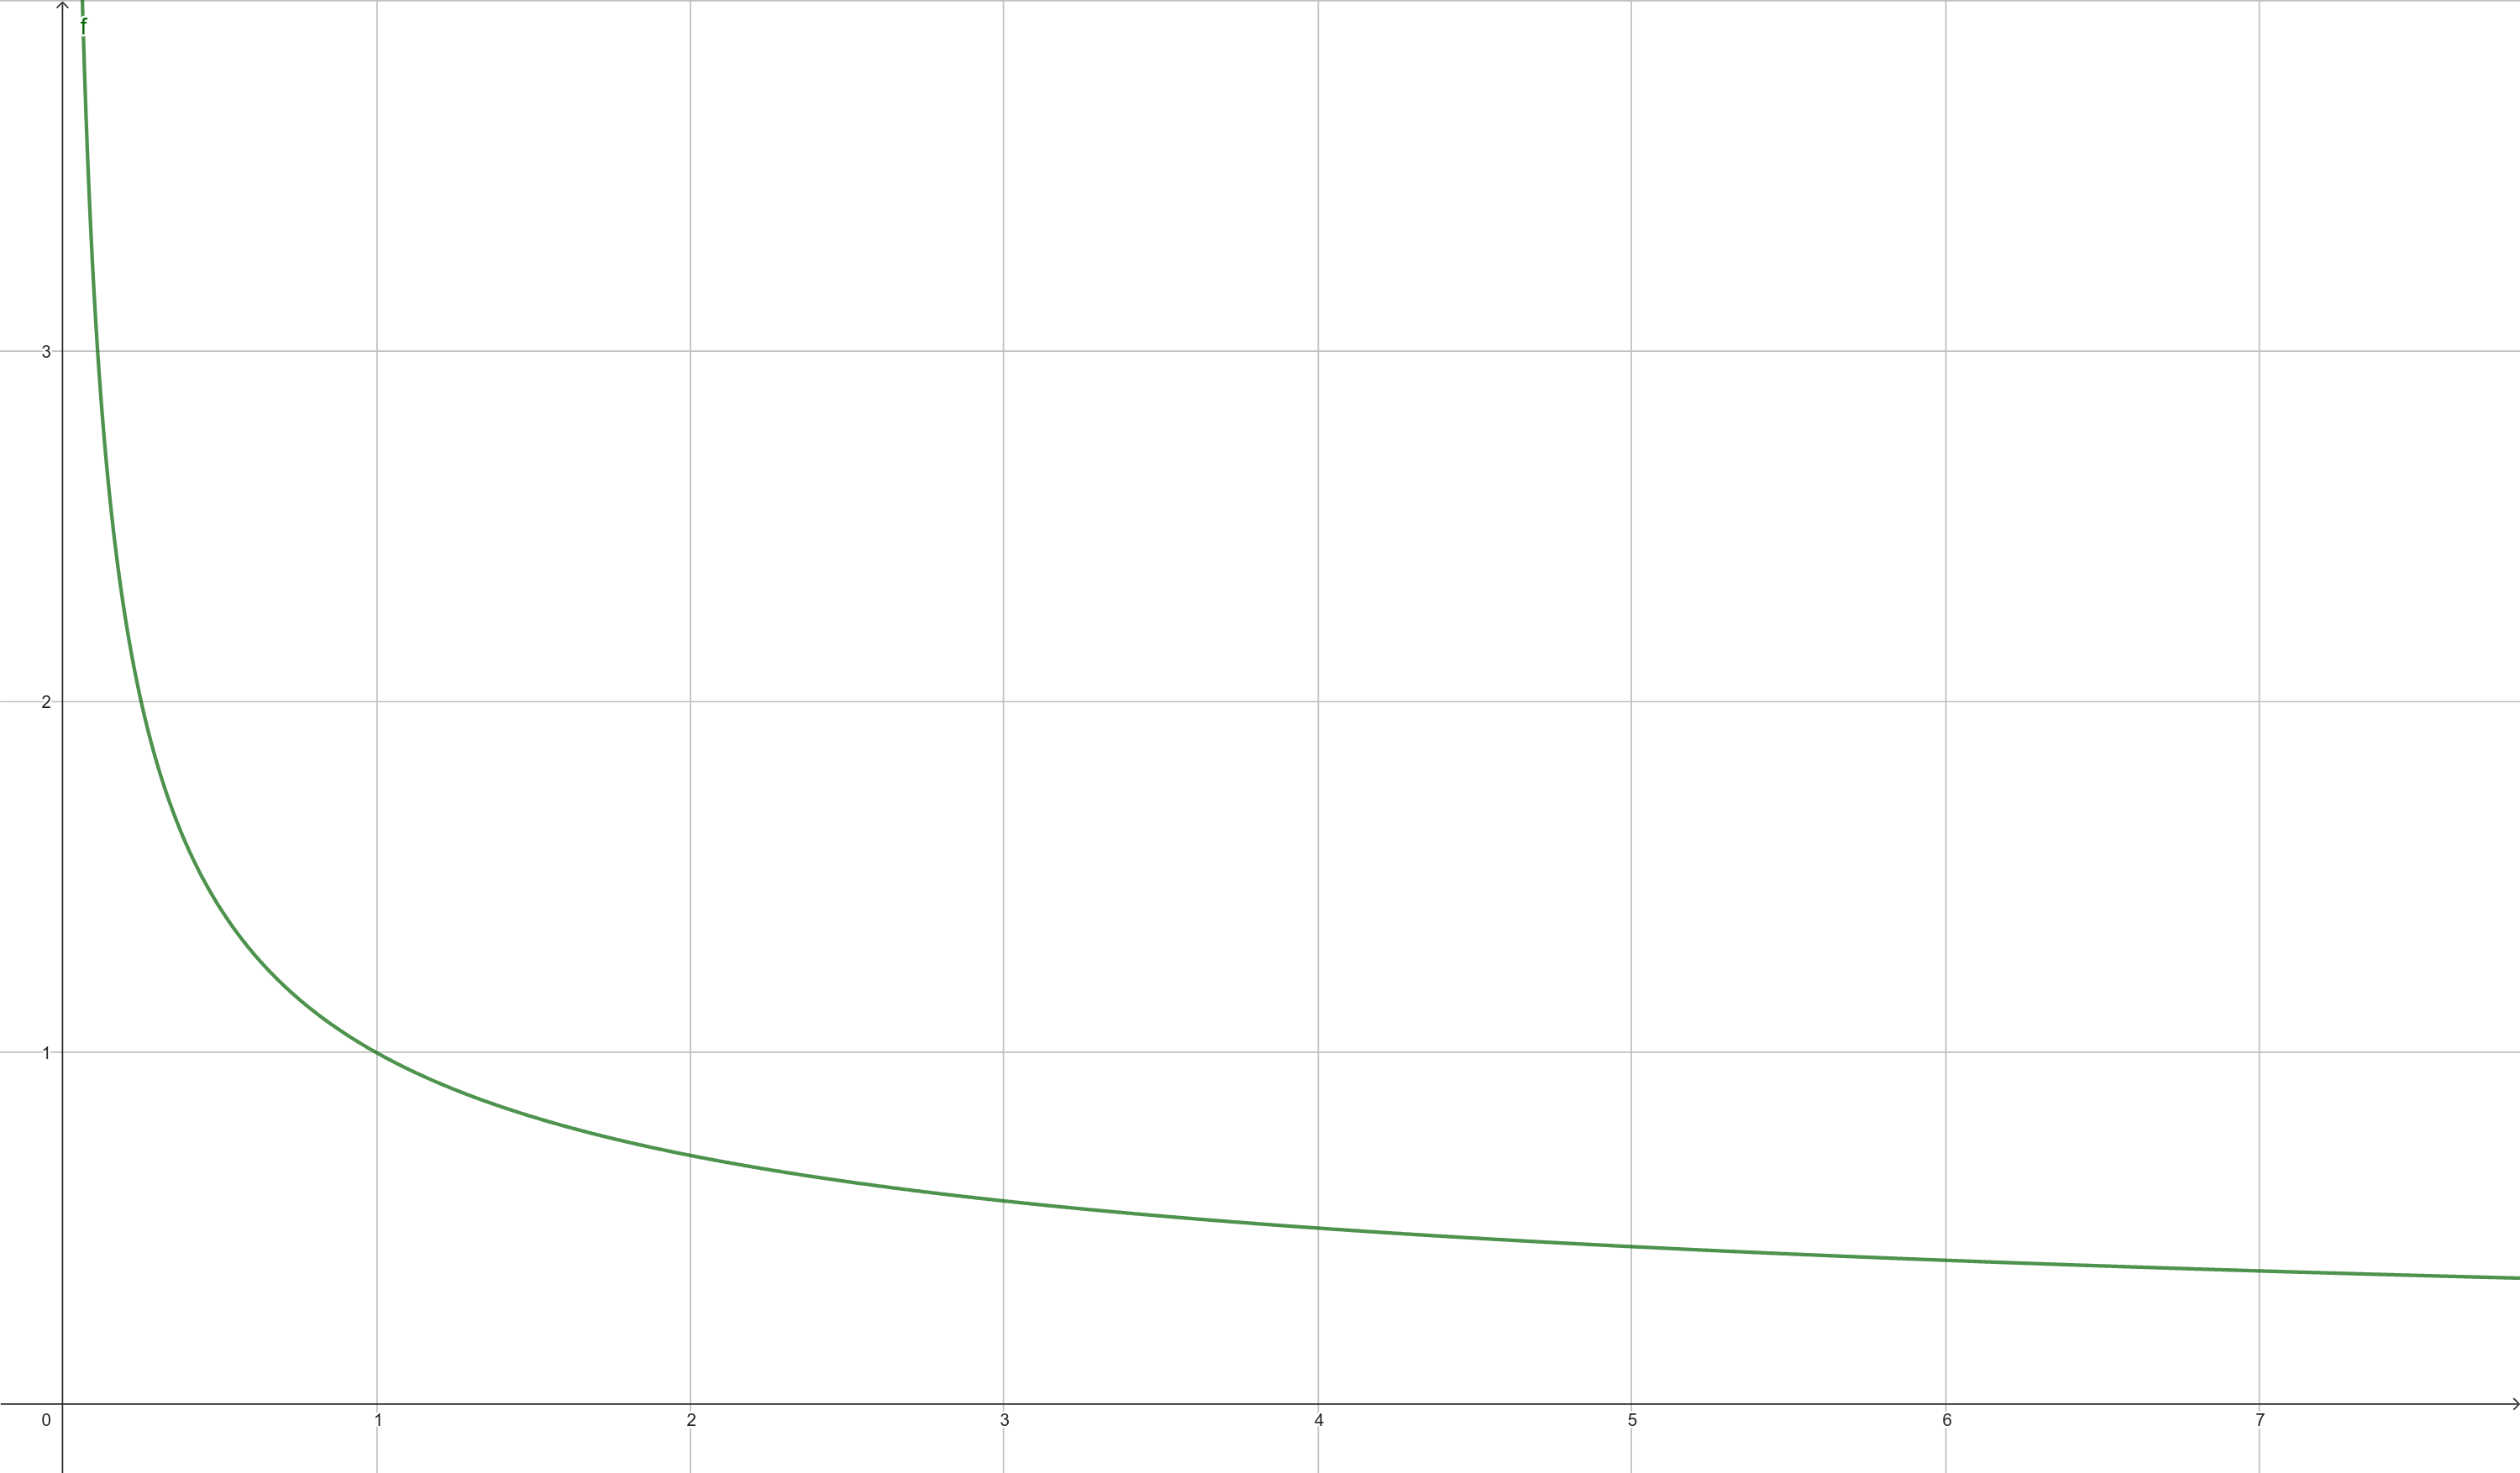
\includegraphics[height=6cm,width=\linewidth]{1_sqrt_x}
    \item(10 pontos) \\
    \(
      \int f(x) \, dx
      = \int \frac{1}{\sqrt{x\,}} dx
      = \int x^{-\sfrac{1}{2}}\, dx
      = \frac{x^{-\sfrac{1}{2}+1}}{-\sfrac{1}{2}+1} + C
      = \frac{x^{\sfrac{1}{2}}}{\sfrac{1}{2}}
      = 2\sqrt{x} + C
    \)
    \item(10 pontos) \\
    \(
      \int_0^4 f(x)\,dx
      = \lim_{a\to 0} \int_a^4  \frac{1}{\sqrt{x\,}} dx
      = \lim_{a\to 0} \left[ 2\sqrt{x} \,\evalat{a}{4}\,\right]
      = \lim_{a\to 0} \left(2\sqrt{4} - 2\sqrt{a}\right)
      = 2\sqrt{4} - 2\sqrt{0}
      = 4
    \)
  \end{enumerate}
\end{resposta}

% 03
%------------------------------------------------------------------------------%
\exercise{25}
Considerando as curvas
\[
  y = \frac{1}{x},
  \qquad
  y = \frac{1}{x^2}
  \qquad\text{e}\qquad
  x = 3
\]
\begin{enumerate}[label=\alph*)]
  \item Esboce o gráfico das curvas e indique a área entre elas
  \item Calcule a área
\end{enumerate}

\begin{resposta}
  \begin{enumerate}[label=\alph*)]
    \item(10 pontos) \\
    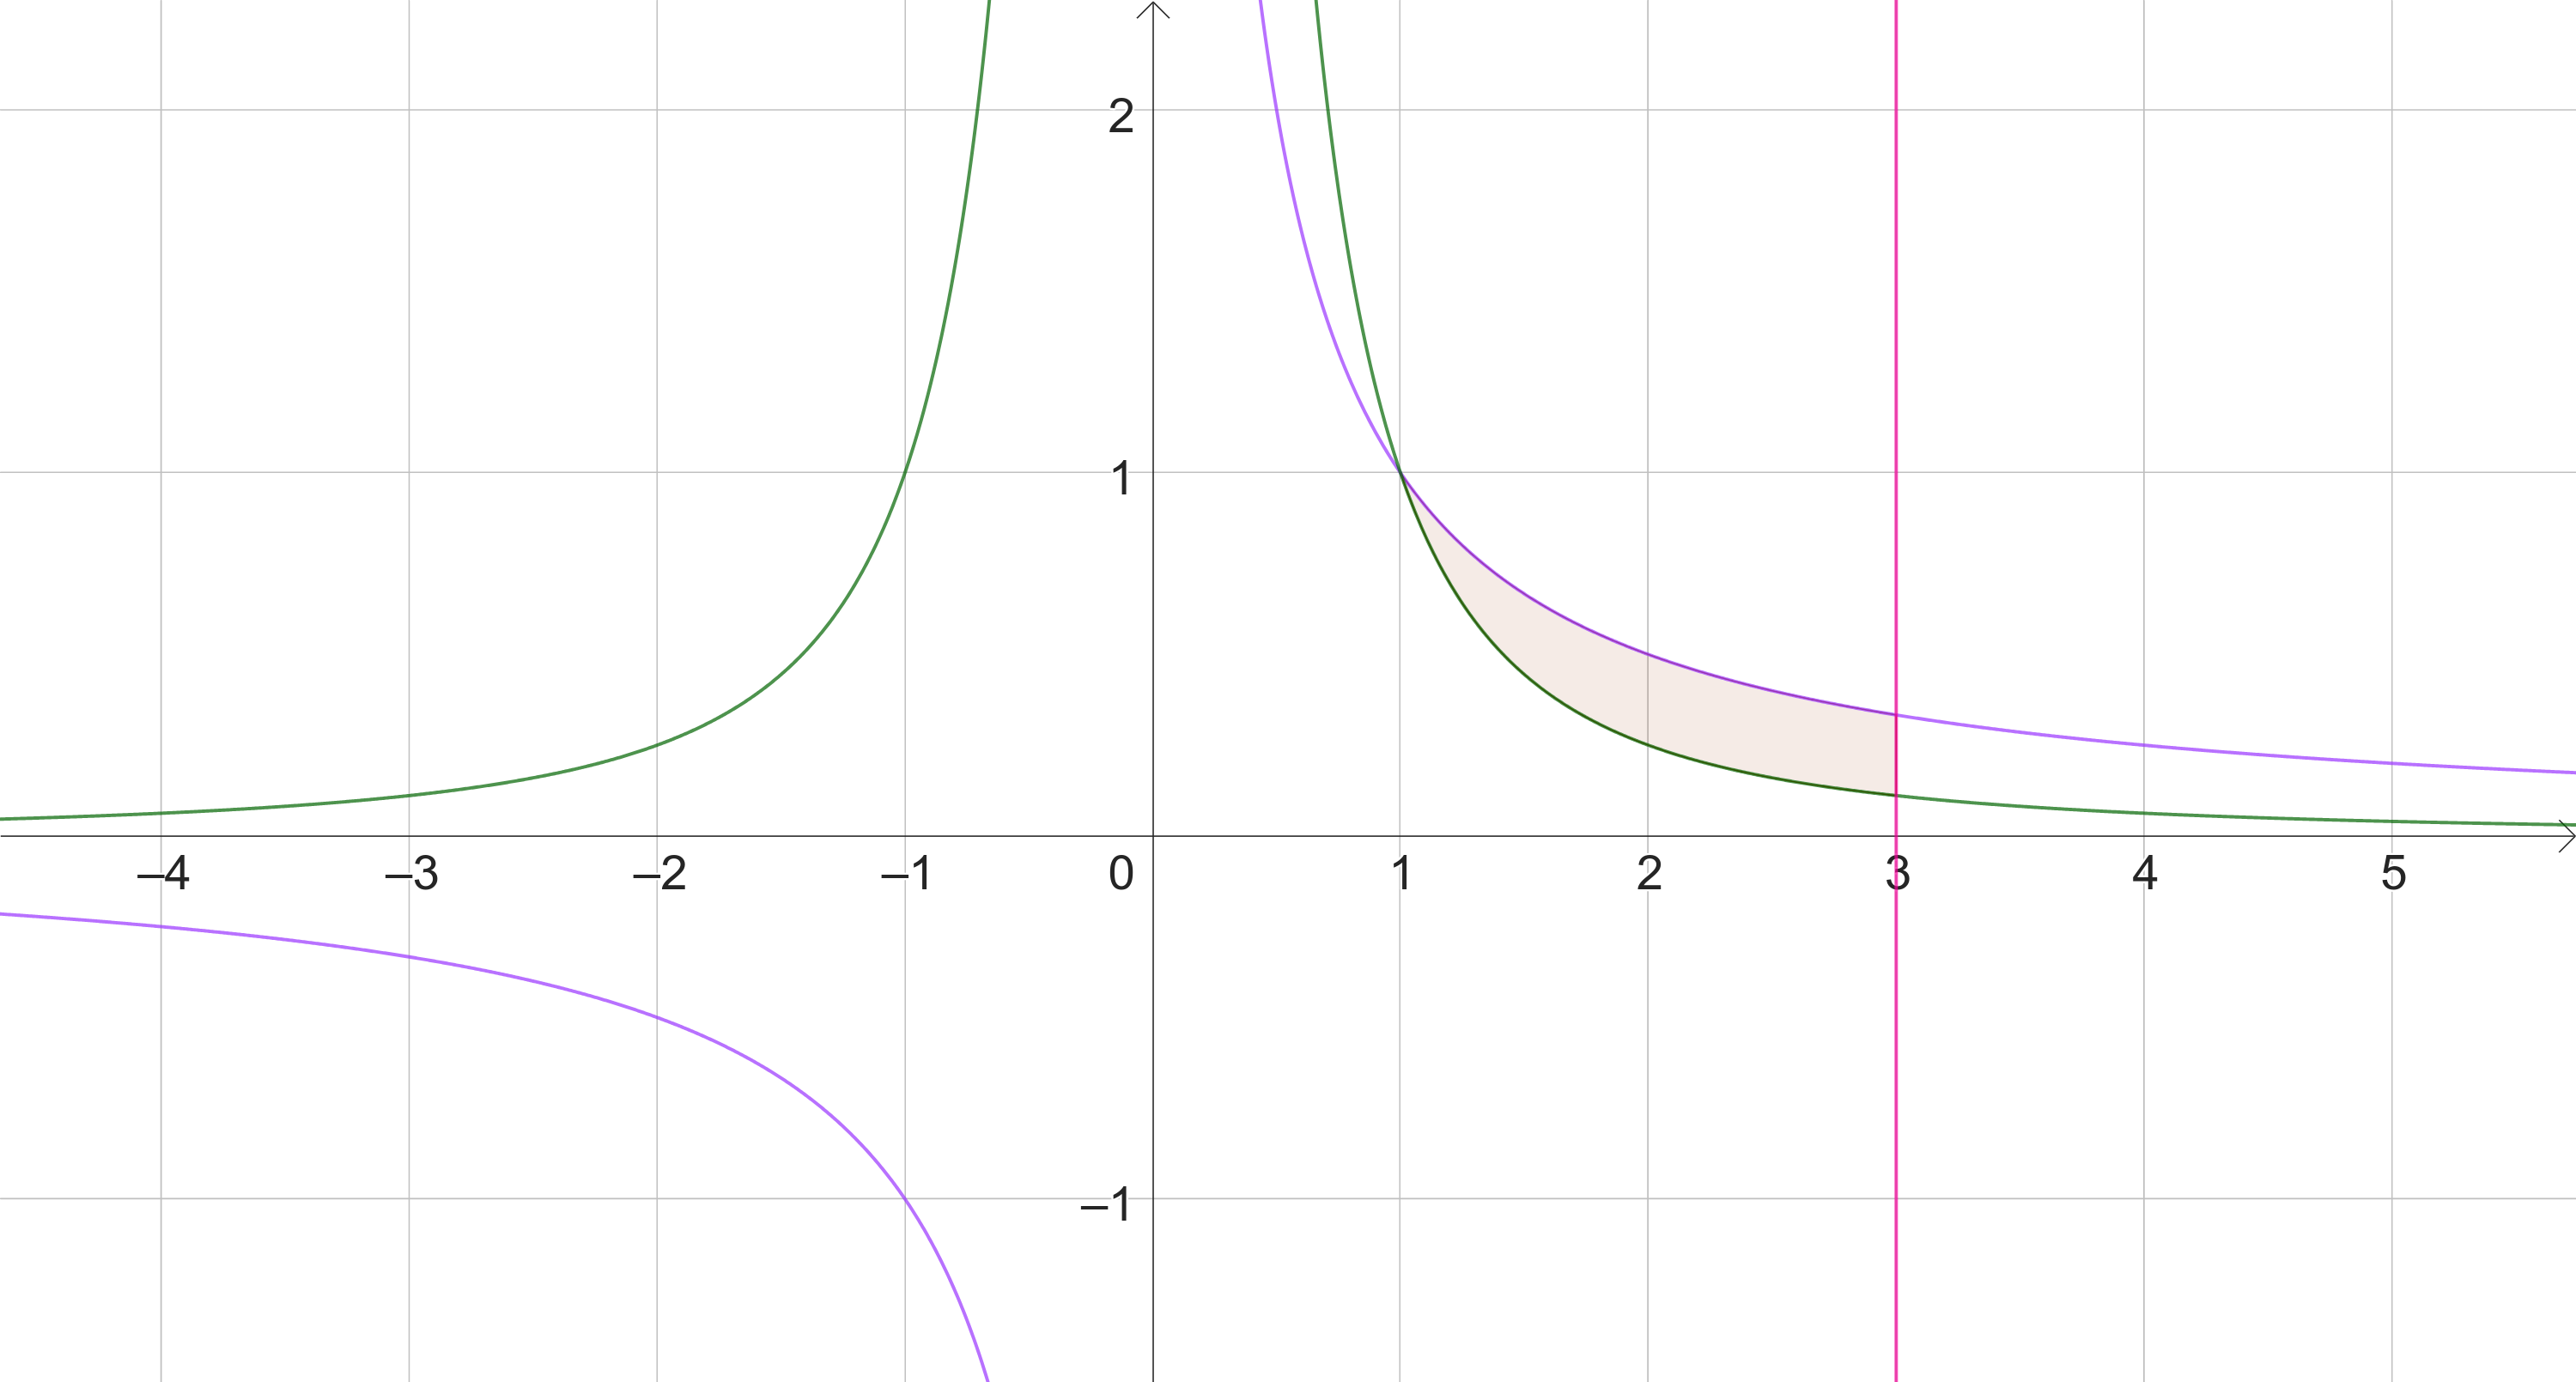
\includegraphics[height=6cm,width=\linewidth]{area_T4}
    \item(15 pontos) \\
    Para encontrar o ponto de interseção resolvemos e equação a seguir sabendo que $x>0$
    \begin{align*}
      \frac{1}{x} & = \frac{1}{x^2} \\
      x^2         & = x             \\
      x           & = 1
    \end{align*}
    Podemos agora calcular a área, sabendo que no intervalo
    \(\frac{1}{x} > \frac{1}{x^2}\)
    \begin{align*}
      A
      & = \int_1^3 \frac{1}{x} - \frac{1}{x^2} \,dx \\
      & = \int_1^3 x^{-1} - x^{-2} \,dx \\
      & = \left( \ln\abs{x} - \frac{x^{-2+1}}{-2+1}\right) \evalat{1}{3} \\
      & = \left( \ln(x) + \frac{1}{x}\right)  \evalat{1}{3} \\
      & = \left( \ln(3) + \frac{1}{3}\right)
        - \left( \ln(1) + \frac{1}{1}\right) \\
      & = \ln(3) + \frac{1}{3} - 1 \\
      & = \ln(3) - \frac{2}{3}
    \end{align*}
  \end{enumerate}
\end{resposta}

% 04
%------------------------------------------------------------------------------%
\exercise{25}
Encontre o volume do sólido obtido pela rotação
da região limitada pelas curvas
\[
  y = \sqrt{x},
  \qquad
  y = 0
  \qquad\text{e}\qquad
  x = 1
\]
em torno da reta
\(
  x = -1
\)

\begin{resposta}
  \centerline{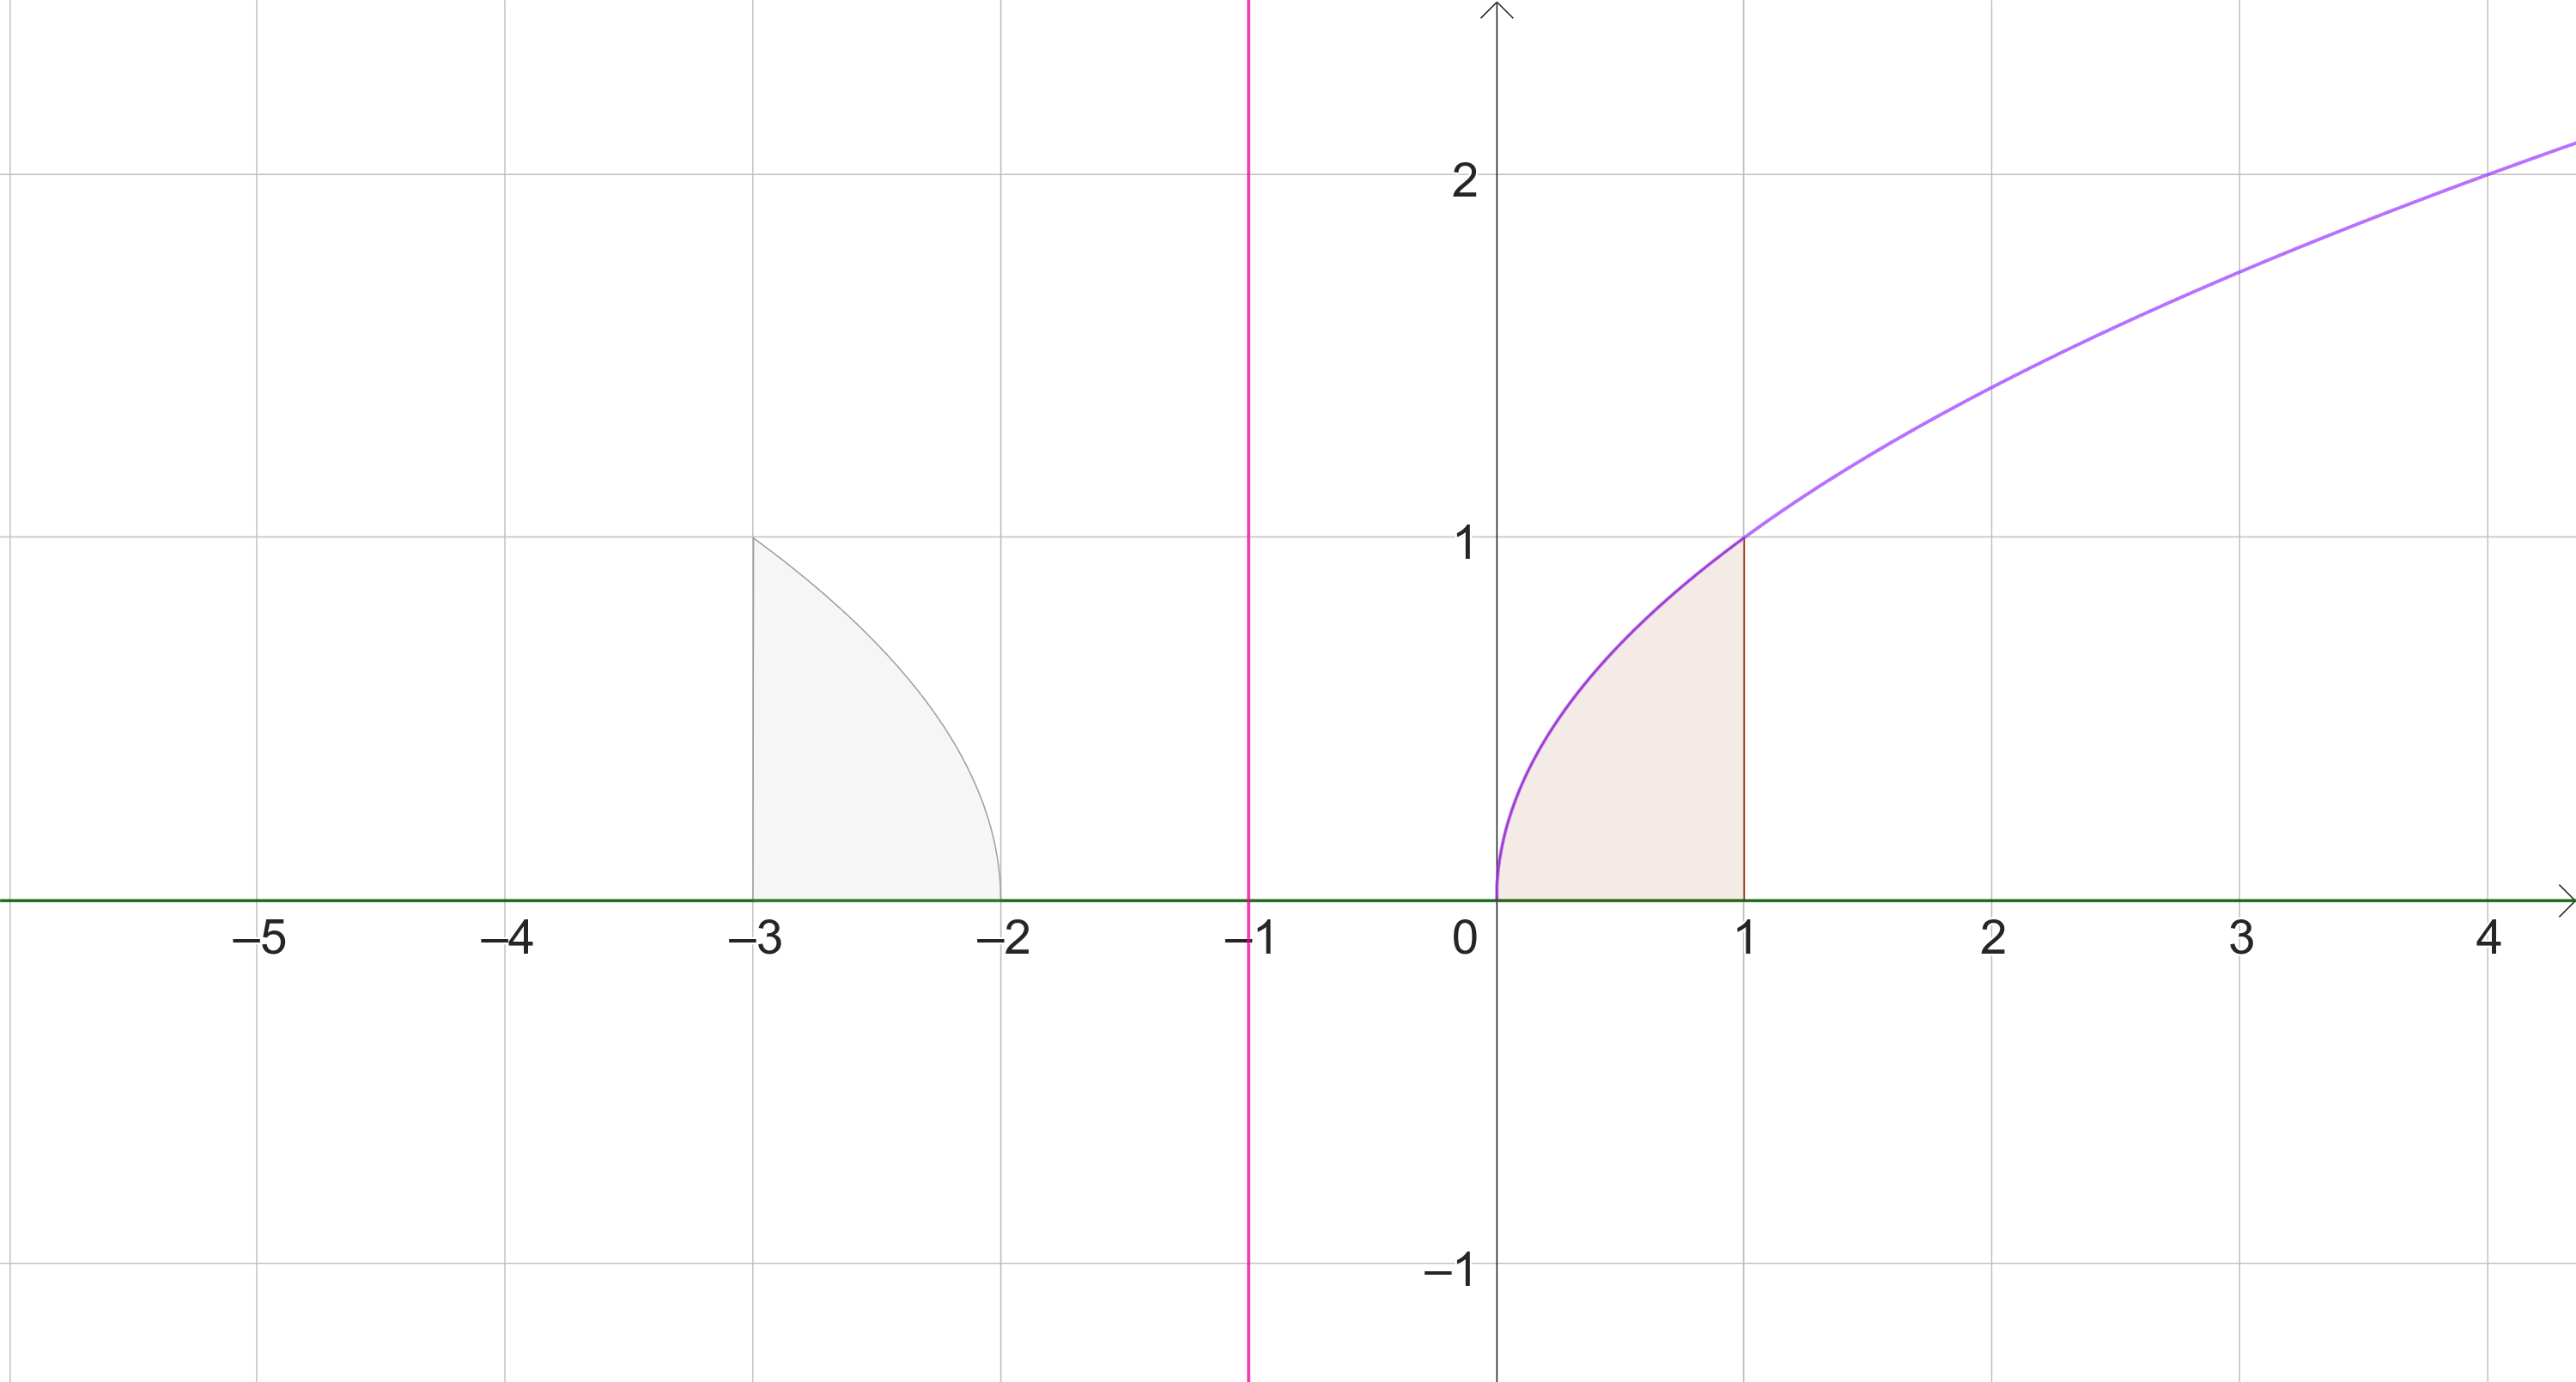
\includegraphics[height=6cm,width=\linewidth]{volume_T4}}

  \vspace{\baselineskip}
  \noindent
  Usando cascas cilíndricas, o volume é dado por
  \[
    V = \int_a^b 2\pi r(x) h(x) \,dx
  \]
  Pelo gráfico verificamos que
  \begin{align*}
    a & = 0 \\
    b & = 1 \\
    r(x) & = x + 1 \\
    h(x) & = \sqrt{x}
  \end{align*}
  Portanto
  \begin{align*}
    V
    & = \int_a^b 2\pi r(x) h(x) \,dx \\
    & = \int_0^1 2\pi (x+1) \sqrt{x} \,dx                  & \text{(15 pontos)}\\
    & = 2\pi \int_0^1 (x+1) x^{\sfrac{1}{2}} \,dx \\
    & = 2\pi \int_0^1 x^{\sfrac{3}{2}} + x^{\sfrac{1}{2}}  \,dx \\
    & = 2\pi \left(
               \frac{x^{\sfrac{3}{2}+1}}{\sfrac{3}{2}+1} +
               \frac{x^{\sfrac{1}{2}+1}}{\sfrac{1}{2}+1}
             \right) \evalat{0}{1} \\
    & = 2\pi \left(
               \frac{2}{5} x^{\sfrac{5}{2}} +
               \frac{2}{3} x^{\sfrac{3}{2}}
             \right) \evalat{0}{1} \\
    & = 2\pi \left[\left(\frac{2}{5} + \frac{2}{3}\right) - 0 \right] \\
    & = 2\pi \frac{6+10}{15} \\
    & = \frac{32\pi}{15} & \text{(10 pontos)}
  \end{align*}
\end{resposta}

%------------------------------------------------------------------------------%
\end{document}
%------------------------------------------------------------------------------%
